\documentclass[10pt,twocolumn,letterpaper]{article}
\usepackage[margin=2.5cm]{geometry}
\usepackage{times,epsfig,graphicx,amsmath,amssymb,float}
\usepackage[breaklinks=true,colorlinks=true,bookmarks=false]{hyperref}
\date{}

%%%%%%%%%%%%%%%%

\title{HDR Image Rendering with refined iCAM06}

\author{%
Hao Sun\\
{\tt wustl-key: sun.hao; email: hao.sun@wustl.edu}
}


\begin{document}
\maketitle

%5 points Presentation
%20 points Report
%	Abstract: 2 pts (One paragraph succinct summary)
%	Introduction/Motivation: 3 pts
%		Why is this problem important, what is the vision task, prelude to rest of the report.
%	Related work: 5 pts 
%		How have other people solved it ? What are other similar problems ? Read, describe.
%	Description / Experiments / Technical Correctness: 7 pts
%	Conclusion: 3 pts

\begin{center}\textbf{Abstract}\\~\\\parbox{0.475\textwidth}{\em
    % Abstract goes here
     The main goal of this project is to research and implement a practical Tone Mapping Operator (TMO) to transfer HDR image to LDR image for laptop display or printing with satisfied performance. In this report, an existing image appearance model, called iCAM06 is introduced, and then improvements are implemented on iCAM06. These improvements includes: using the guided filtering instead of the bilateral filtering to convert the input data into detail layer and base layer; using an modified chromatic adaption matrix CAT02 to make tone mapped images more similar to human eye perception. Experimental results show that the refined iCAM06 model improve the performance of HDR image rendering.

}\end{center}

\section{Introduction}
Scenes in real-world environment usually have extremely wide range of light luminance from very bright, direct sunlight to extreme shade (up to 9 log units). Human eye is so complicated and subtle to handle this condition, so as kinds of imaging technology with High Dynamic Range (HDR). However, traditional Low Dynamic Range(LDR) display devices as well as hardcopy prints cannot fully display HDR image information. So, HDR rendering algorithms, which are also known as Tone Mapping Operators (TMOs) are designed to scale the wide range of luminance information that exists in the real world so that it can be displayed on a device that is only capable of producing a much lower dynamic range\cite{kuang2007icam06}.

Tone Mapping is a technique used mapping one set of colors to another so that to approximate the appearance of high-dynamic-range images in a medium that has a more limited dynamic range. It is widely used in image processing and computer graphics. Print-outs, CRT or LCD monitors, and projectors all have a limited dynamic range that is inadequate to reproduce the full range of light intensities present in natural scenes. Tone mapping addresses the problem of strong contrast reduction from the scene radiance to the displayable range while preserving the image details and color appearance important to appreciate the original scene content, an example of tone mapping is shown in figure \ref{tone mapping}.

The goal of Tone Mapping in HDR rendering applications is to obtain a perceptual match between a real scene and a displayed image even though the display device is not able to reproduce the full range of luminance values. This report introduces a commonly used Tone Mapping algorithm named iCAM06 which is based on both the color appearance model and hierarchical mapping\cite{krawczyk2005lightness}. In the next section, the background and related work of Tone Mapping will be introduced; in the third section, the framework and process of iCAM06 will be 
explained in detail; in the fourth section, experiments based on iCAM06 will be conducted; the last part is the conclusion of this report.

\begin{figure}[!t]
\begin{center}
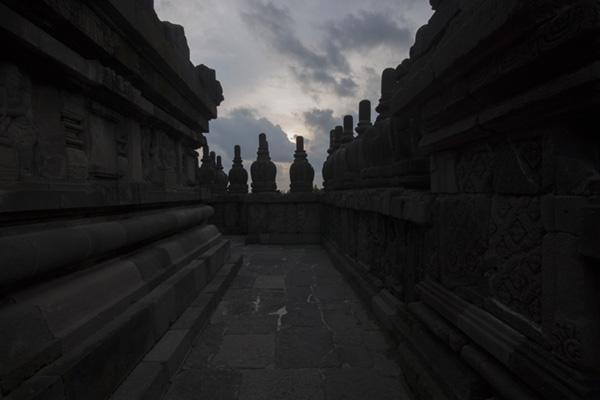
\includegraphics[height=15em]{images/original_HDRimage.jpg}
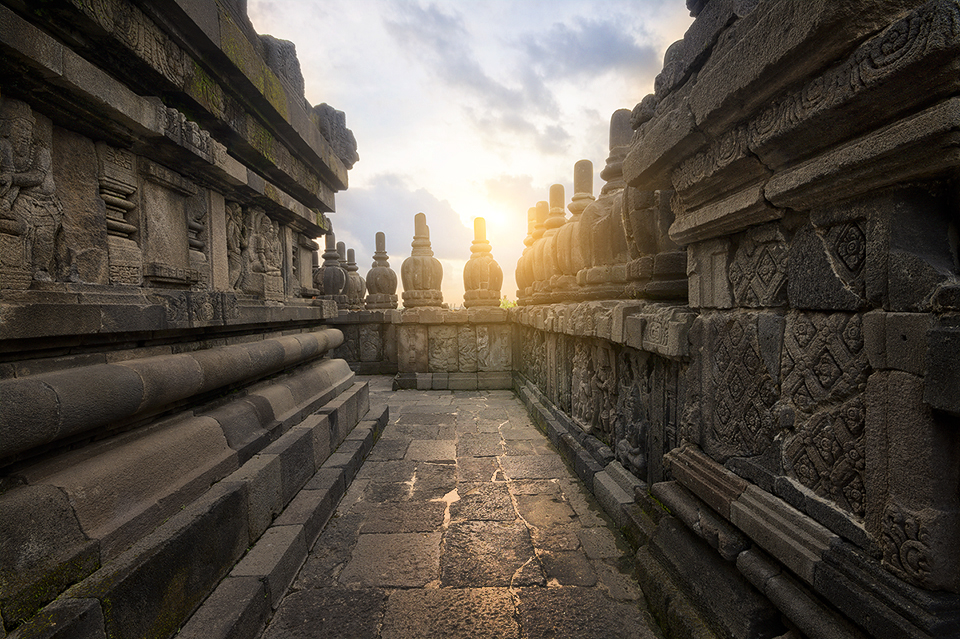
\includegraphics[height=15em]{images/toned_image.jpg}
\end{center}
   \caption{Tone Mapping for HDR image. (Prambanan Temple by Jimmy McIntyre)}
\label{tone mapping}
\end{figure}

\newpage
\begin{figure*}[!tp]
	\begin{center}
	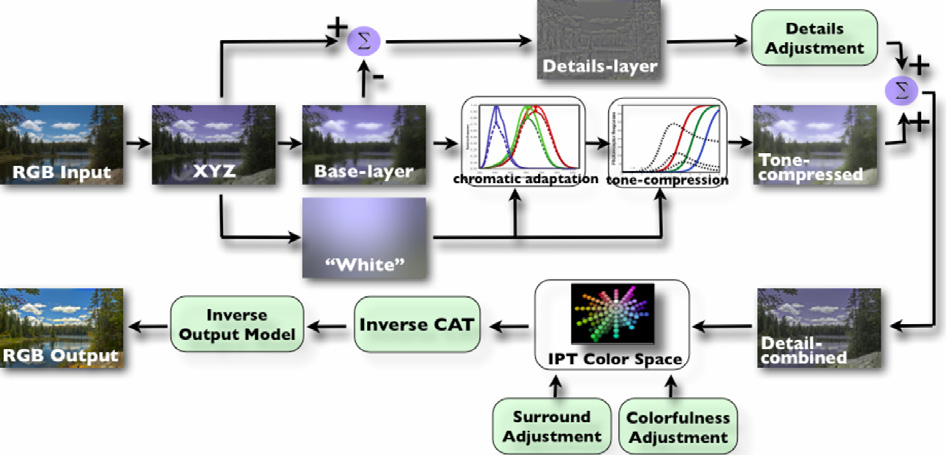
\includegraphics[height=15em]{images/iCAM06_Framework.jpg}
	\end{center}
   	\caption{Framework of iCAM06 model.}
  	\label{iCAM06_Framework}
\end{figure*}

\section{Background \& Related Work}
TMO is derived from the issues created by file-based photography. Capturing the wide dynamic range of luminance from the real world on a chemically limited negative was very difficult, and early film developers attempted to remedy this issue by designing the film stocks and the print development systems that gave a desired S-shaped tone curve with slightly enhanced contrast (about 15\%) in the middle range and gradually compressed highlights and shadows\cite{livingstone2002vision}. Photographers have also used dodging and burning to overcome the limitations of the print process\cite{hunt1987reproduction}.

Then, the birth of digital photography brought hope to better solving this problem. Retinex, employed by Land and McCann in 1971, is one of the earliest algorithms\cite{adams1981print}.This algorithm is inspired by the eye's biological mechanisms of adaptation when lighting conditions are changing. Various TMOs have been developed in the recent years. There are mainly three types:
\begin{itemize}
\item Global (or spatially uniform) operators: they are non-linear functions based on the luminance and other global variables that are spatially independent. Once the optimal function has been estimated according to the particular image, every pixel in the image is mapped in the same way, independent of the value of surrounding pixels in the image\cite{qiu2006tone}. Those techniques are simple and fast, and they can maintain the overall brightness contrast of the image but they can cause a loss of details. Examples of common global tone mapping methods are contrast reduction and color inversion.

A simple example of global tone mapping filter is $V_{out} = \frac{V_{in}}{V_{in} + 1}$, where $V_{in}$ is the luminance of the original pixel and $V_{out}$ is the luminance of the filtered pixel\cite{reinhard2002photographic}. This function will map the luminance $V_{in}$ in the range of $\lbrack0,\infty)$ to a displayable output range of $\lbrack0,1)$. While the filter provides a decent contrast for parts of the image with low luminance (particularly when $V_{in} < 1$), parts of the image with high luminance will get lower contrast. Another useful global tone mapping is gamma compression, which has a filter $V_{out} = AV_{in}^\gamma$, where $A>0$and$0<\gamma<1$. This function will map the luminance $V_{in}$ in the range of $[0,1/A^{1/\gamma}]$ to the output range of $[0,1]$.$\gamma$regulates the contrast of the image: a lower value for lower contrast. While a lower constant $\gamma$ gives a lower contrast and perhaps also a duller image, it increases the exposure of underexposed parts of the image. If $A<1$, it can decrease the exposure of overexposed parts of the image.


\item Local (or spatially varying) operators: the parameters of the non-linear function change in each pixel, based on its spatial information. Parameters change according to features extracted from the surrounding parameters. In other words, the effect of the algorithm changes in each pixel according to the local features of the image. Those algorithms are more complicated than the global ones; they can show artifacts (e.g. halo effect and ringing); and the output can look unrealistic, but if used correctly, they can provide the best performance, because human vision is mainly sensitive to local contrast.

Local tone mapping algorithms are based on contrast or gradient domain. Such TMOs concentrate on preserving contrast between neighboring regions rather than absolute value, an approach motivated by the fact that human perception is most sensitive to contrast in images rather than absolute intensities. Those tone mapping methods usually produce very sharp images, which preserve very well small contrast details; however, this is often done at the cost of flattening an overall image contrast, and may as a side effect produce halo-like glows around dark objects\cite{devlin2002star}.

\item Color appearance model: the commonly used one is iCAM(image color appearance model), which is based on the color appearance model and hierarchical mapping\cite{fairchild2004icam}, it attempts to predict perceptual responses to spatially complex stimuli. As such, they can provide a unique framework for the prediction of the image appearance of HDR image. In 2003, iCAM tone mapping algorithm was proposed\cite{johnson2003rendering}. Based on the iCAM framework, the iCAM06 model was developed for HDR image rendering. A number of improvements (e.g. Gaussian filter was replaced by bilateral filter in iCAM06) have been implemented in iCAM06 on the motivation of a better algorithm that is capable of providing more perceptually accurate HDR renderings and a more developed perceptual model for a wide range of image appearance prediction\cite{kuang2007icam06}. 

\end{itemize}

\section{Framework of the iCAM06 model}

The goal of the iCAM06 model is to accurately predict human visual attributes of complex images in a large range of luminance levels and thus reproduce the same visual perception across media. The framework of iCAM06 for HDR image rendering is shown in figure \ref{iCAM06_Framework}. 

\subsection{Input data}
\label{sec:parta}
The input data for iCAM06 model are CIE tri-stimulus values (that is XYZ image) for the stimulus image or scene in absolute luminance units. Y is the absolute luminance of the image, it is necessary to predict various luminance-dependent phenomena, such as the Hunt effect and the Stevens effect. A RGB encoded image can be transformed into CIE 1931 XYZ tri-stimulus values through the specific camera characterization and an example transformation using the sRGB color space transform matrix is shown in the following equation:

\begin{align}
	\left[
		\begin{array}{c}
		X\\
		Y\\
		Z
		\end{array}
	\right]
	= M_{sRGB}
	\left[
		\begin{array}{c}
		R\\
		G\\
		B
		\end{array}
	\right]\\
	M_{sRGB} = 
	\left[
		\begin{array}{ccc}
		0.4124&0.2127&0.0193\\
		0.3576&0.7152&0.1192\\
		0.1805&0.0722&0.9504
		\end{array}
	\right]
\end{align}

\subsection{Image decomposition}
\label{sec:partb}
After the input image is transformed to XYZ image, the image is decomposed into a base-layer and a detail layer. The chromatic adaption and tone-compression are applied to the base layer, so the details of the image will be preserved. The two-scale decomposition is motivated by two widely accepted assumptions in human vision: (1) An image is regarded as a product of the reflectance and the illumination, and human vision is mostly sensitive to the reflectance rather than the illumination conditions; (2) human vision responses mostly to local contrast instead of the global contrast\cite{kuang2007icam06}. The fact that the human visual system is insensitive to the global luminance contrast enables the solution of compressing the global dynamic range and preserving local details in an scene with HDR, so as to reproduce the same perceptual appearance on a display device with LDR.

This model uses bilateral filter to obtain base-layer image. Bilateral filter is a non-linear one, and each pixel is the product of its neighbor's intensity and weight which is determined by the product of the distance between this pixel and the neighbor and the intensity difference. Therefore, bilateral filter effectively blurs an image and keeps sharp edges in the meantime. The output of the bilateral filter for a pixel $s$ is expressed in the following equations:

\begin{align}
	J_s = \frac{1}{K(s)}\sum_{}^{}f(p-s)g(I_p-I_s)I_p\\
	k(s) = \sum_{}^{}f(p-s)g(I_p-I_s)
\end{align}
Where k(s) is a normalization term, $p$ is the neighbor of $s$, $f()$ is a Gaussian function in the spatial domain with the kernel scale $\sigma_s$ set to empirical value of 2\% of the image size, and $g()$ is another Gaussian function in the intensity domain with its scale $\sigma_r$ set to a constant value of 0.35\cite{durand2002fast}. $I_s$ is the intensity of pixel $s$, which will get more value from neighbor pixels that are close spatially and that have a similar intensity.

By subtracting the base layer image from the original image, the detail layer can be obtained. In the following processing, these two layer images will be transformed back to RGB.

\subsection{Chromatic adaption}
\label{sec:partc}
Chromatic adaption is a linear von Kries normalization of the spectral sharpened RGB image with the help of RGB adaption white image which is derived from the Gaussian low-pass adaptation image at each pixel location $(R_wG_wB_w)$. The amount of blurring in the low-pass image is determined by the half-width of the filter $\sigma$, which is suggested to set as 5-degree radius of background\cite{yamaguchi2004study}. The conditions of the viewing are often unknown for the process of HDR image rendering, thus the width of the filter can be specified based on the image size itself. Before chromatic adaption XYZ image should be transformed back to RGB image using $M_{CAT02}$, and the operation of chromatic adaption is shown as follows:
\begin{flalign}
	\left[
		\begin{array}{c}
		R\\
		G\\
		B
		\end{array}
	\right]
	= M_{CAT02}
	\left[
		\begin{array}{c}
		X\\
		Y\\
		Z
		\end{array}
	\right]\\
	M_{CAT02} = 
	\left[
		\begin{array}{ccc}
		0.7328&0.4296&-0.1624\\
		-0.7036&1.6975&0.0061\\
		0.0030&0.0136&0.9834
		\end{array}
	\right]\\
	D=0.3F[1-(\frac{1}{3.6})e^{(\frac{-(L_A-42)}{92}))}]\\
	R_c = [(R_{D65}\frac{D}{R_W})+(1-D)]R\\
	G_c = [(G_{D65}\frac{D}{G_W})+(1-D)]G\\
	B_c = [(B_{D65}\frac{D}{B_W})+(1-D)]B
\end{flalign}
In the beginning of the transformation, a conversion from CIE XYZ image to the spectrally sharpened RGB image is done by using the matrix $M_{CAT02}$. $D$ is the incomplete adaptation factor, which is computed as a function fo adaption luminance $L_A$ (20\% of the adaptation white) and surround factor $F$ ($F=1$ in an average surround). In practice, the minimum value is 0.65 for a dark surround and exponentially converge to 1 with an increasing $L_A$. In iCAM06, a scale factor of 0.3 is used in order to reduce the color de-saturation for HDR image rendering.


\subsection{Tone compression}
\label{sec:partd}
The process of tone compression is a simulation of the photoreceptor responses, including cones and rods. Therefore, the tone compression output of iCAM06 is a combination of cone response and rod response.

The RGB responses derived from chromatic adaption should be first converted from the CAT02 space to Hunt-Pointer-Estevez fundamentals by using the CIECAM02 formula:

\begin{equation}
	\left[
		\begin{array}{c}
		R'\\
		G'\\
		B'
		\end{array}
	\right]
	= M_{HPE}M_{CAT02}^{-1}
	\left[
		\begin{array}{c}
		R_C\\
		G_C\\
		B_C
		\end{array}
	\right]
\end{equation}

\begin{equation}
M_{HPE} = 
	\left[
		\begin{array}{ccc}
		0.38971&0.68898&-0.07868\\
		-0.22981&1.18340&0.04641\\
		0.0&0.0&1.0
		\end{array}
	\right]
\end{equation}

\begin{equation}
M_{CAT02}^{01} = 
	\left[
		\begin{array}{ccc}
		1.096124&-0.278869&0.182745\\
		0.454369&0.473533&0.072098\\
		-0.009628&-0.005698&1.015326
		\end{array}
	\right]
\end{equation}
The cone response prediction has a good performance on all available visual data. The nonlinear cone response functions are shown in the following equations. The $p$ is a user-controllable variable, which can be set in the range of 0.6-0.85, where the larger value generates higher overall contrast in the output image. A default value is 0.75.


\begin{equation}
	R'_a = \frac{400(F_LR'/Y_W)^p}{27.13+(F_LR'/Y_W)^p}+0.1
\end{equation}

\begin{equation}
	G'_a = \frac{400(F_LG'/Y_W)^p}{27.13+(F_LG'/Y_W)^p}+0.1
\end{equation}

\begin{equation}
	B'_a = \frac{400(F_LB'/Y_W)^p}{27.13+(F_LB'/Y_W)^p}+0.1\\
\end{equation}

\begin{equation}
	F_L=0.2k^4(5L_A)+0.1(1-k^4)^2(5L_A)^{1/3}
\end{equation}

\begin{equation}
	k=1/(5L_A+1)
\end{equation}

In CIECAM02 and other earlier models, the $F_L$ function is used to predict a variety of luminance-dependent appearance effects. However, the computation of the $F_L$ factor in iCAM06 is different from that in the previous color appearance models, because it is derived from the low-pass adaptation image at each pixel location and thus spatially varied in iCAM06. $Y_w$ is the luminance of the local adapted white image.

The functions of rod response prediction after adaptation are adapted from Hunt Model\cite{hunt1967reproduction}. The nonlinear response functions is same as that for the cone response, they are shown as follows:

\begin{equation}
	A_s = 3.05B_s[\frac{400(F_{LS}S/S_w)^p}{27.13+(F_{LS}S/S_w)^p}] + 0.3
\end{equation}

\begin{equation}
	F_{LS}=3800j^2(5L_{AS}/2.26)+0.2(1-j^2)^4(5L_{AS}/2.26)^{1/6}
\end{equation}

\begin{equation}
	L_{AS}=2.26L_A
\end{equation}

\begin{equation}
	j=0.00001/[(5L_{AS}/2.26)+0.00001]
\end{equation}

\begin{align}
\begin{aligned}
	B_S = 0.5/\{1+0.3[(5L_{AS}/2.26)(S/S_w)]^{0.3}\}\\
		+0.5/\{1+5[5L_{AS}/2.26]\}
\end{aligned}
\end{align}

$S$ is the luminance of each pixel in the chromatic adapted image and $S_w$ is the value of $S$ for the reference white. By setting $S_w$ to a global scale from the maximum value of the local adapted white point image, the rod response output is automatically adjusted by the general luminance perception of the scene. For example, the rod responses for a bright scene become significantly small comparing to the cone responses in this case. $L_{AS}$ is the scotopic luminance, $B_S$ is the rod pigment bleach or saturation factor, and $F_{LS}$ is the scotopic luminance level adaptation factor.

The final tone compression response is the sum of the cone and rod response:
\begin{equation}
	RGB_{TC} = RGB'_a+A_S
\end{equation}

\subsection{IPT transformation}
\label{sec:parte}
After obtained tone-compressed RGB image, it should be converted back to CIE XYZ image, and combined with the detail layer image. The tone-mapped image is then converted into IPT uniform opponent color space, where $I$ is the lightness channel, $P$ is roughly analogous to a red-green channel, and $T$ is a blue-yellow channel.

The opponent color dimensions and image attributes, such as lightness, hue, and chroma, can be derived from IPT fundamentals for image difference and image quality predictions. For HDR image rendering application, the perceptual uniformity of IPT is also necessary for the desired image attribute adjustments without affecting other attributes. The $XYZ$ units are first converted into LMS cone responses, followed by a nonlinear power function compression, then converted into IPT units. The transformation are following:

\begin{align}
\begin{aligned}
	\left[
		\begin{array}{c}
		L\\
		M\\
		S
		\end{array}
	\right]
	= M_{H}^{D65}
	\left[
		\begin{array}{c}
		X_c\\
		Y_c\\
		Z_c
		\end{array}
	\right]\\
	M_{H}^{D65} = 
	\left[
		\begin{array}{ccc}
		0.4002&0.7075&-0.0807\\
		-0.2280&1.1500&0.0612\\
		0.0000&0.0000&0.9184
		\end{array}
	\right]
\end{aligned}
\end{align}

\begin{align}
\begin{aligned}
	L'=L^{0.43}\\
	M'=M^{0.43}\\
	S'=S^{0.43}
\end{aligned}
\end{align}

\begin{align}
\begin{aligned}
	\left[
		\begin{array}{c}
		I\\
		P\\
		T
		\end{array}
	\right]
	= M_{IPT}
	\left[
		\begin{array}{c}
		L'\\
		M'\\
		S'
		\end{array}
	\right]\\
	M_{IPT} = 
	\left[
		\begin{array}{ccc}
		0.4000&0.4000&0.2000\\
		4.4550&-4.8510&0.3960\\
		0.8056&0.3572&-1.1628
		\end{array}
	\right]
\end{aligned}
\end{align}


\subsection{Image attribute adjustments and image output}
\label{sec:partf}
In iCAM06, there are three attribute adjustments to be implemented to effectively predict image appearance effects. The adjustment in detail-layer processing is applied to predict the Stevens effect, which means an increase in luminance level results in an increase in local perceptual contrast. The adjustment is given as follows:

\begin{equation}
	Details_a = Details^{(F_L+0.8)^{0.25}}
\end{equation}

In the IPT color space, $P$ and $T$ are enhanced to predict the Hunt effect, which predict the phenomenon that an increase in luminance level results in an increase in perceived colorfulness. The adjusted $P$ and $T$ are functions of the $F_L$ factor introduced before and the chroma value, given as the following:
\begin{equation}
	P=P[(F_L+1)^{0.2}(\frac{1.29C^2-0.27C+0.42}{C^2-0.31C+0.42})]
\end{equation}

\begin{equation}
	T=T[(F_L+1)^{0.2}(\frac{1.29C^2-0.27C+0.42}{C^2-0.31C+0.42})]
\end{equation}

Both functions are monotonically increasing, indicating that the colorfulness of low chroma and low luminance color are more preserved than other colors. Since natural objects often have low chroma, this enhancement preserves the natural appearance of these objects.

The perceived image contrast increases when the image surround is changed from dark to dim to light. This effect is predicted using power functions with exponent values of 1, 1.25, 1.5 for dark, dim and average surround respectively\cite{hunt1967reproduction}. To compensate these changes, a power function is applied to I channel of IPT space with exponents in the reverse order as above description:
\begin{align}
\begin{aligned}
	I_a = I^{\gamma}\\
	where \gamma_{dark} = 1.5, \gamma_{dim} = 1.25, \gamma_{average} = 1.0
\end{aligned}
\end{align}

To display the rendered image on an output device, the IPT image should be first converted back to CIE XYZ image, followed by an inverted chromatic adaption transform, from D65 to the output media white point. The inverse output characterization model then is used to transfromed XYZ values to the linear device dependent RGB values.

\section{Experimental Results}
In this part, iCAM06 was applied for rendering three HDR example images, the results are shown as the following figures:

\begin{figure}[H]
\begin{center}
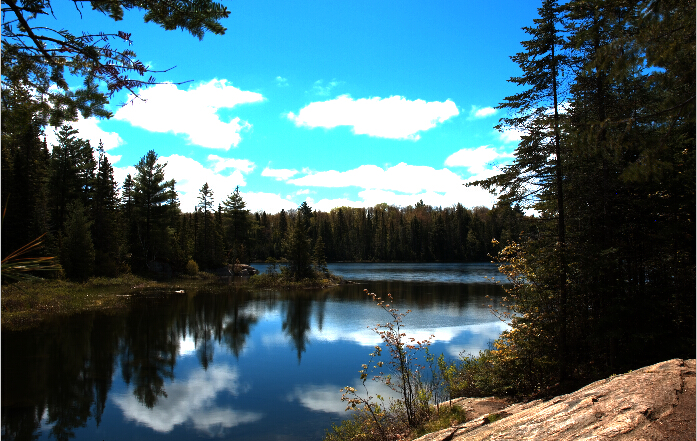
\includegraphics[height=14em]{images/peaklake_original.jpg}
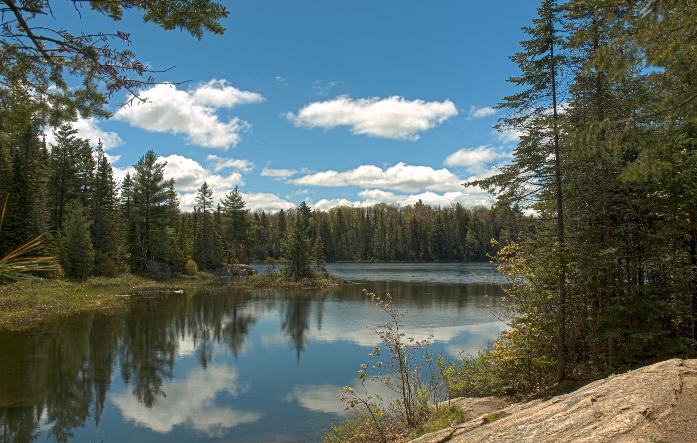
\includegraphics[height=14em]{images/PeckLakegf4.jpg}
\end{center}
   \caption{HDR image rendering 1}
\label{example1}
\end{figure}

\begin{figure}[H]
\begin{center}
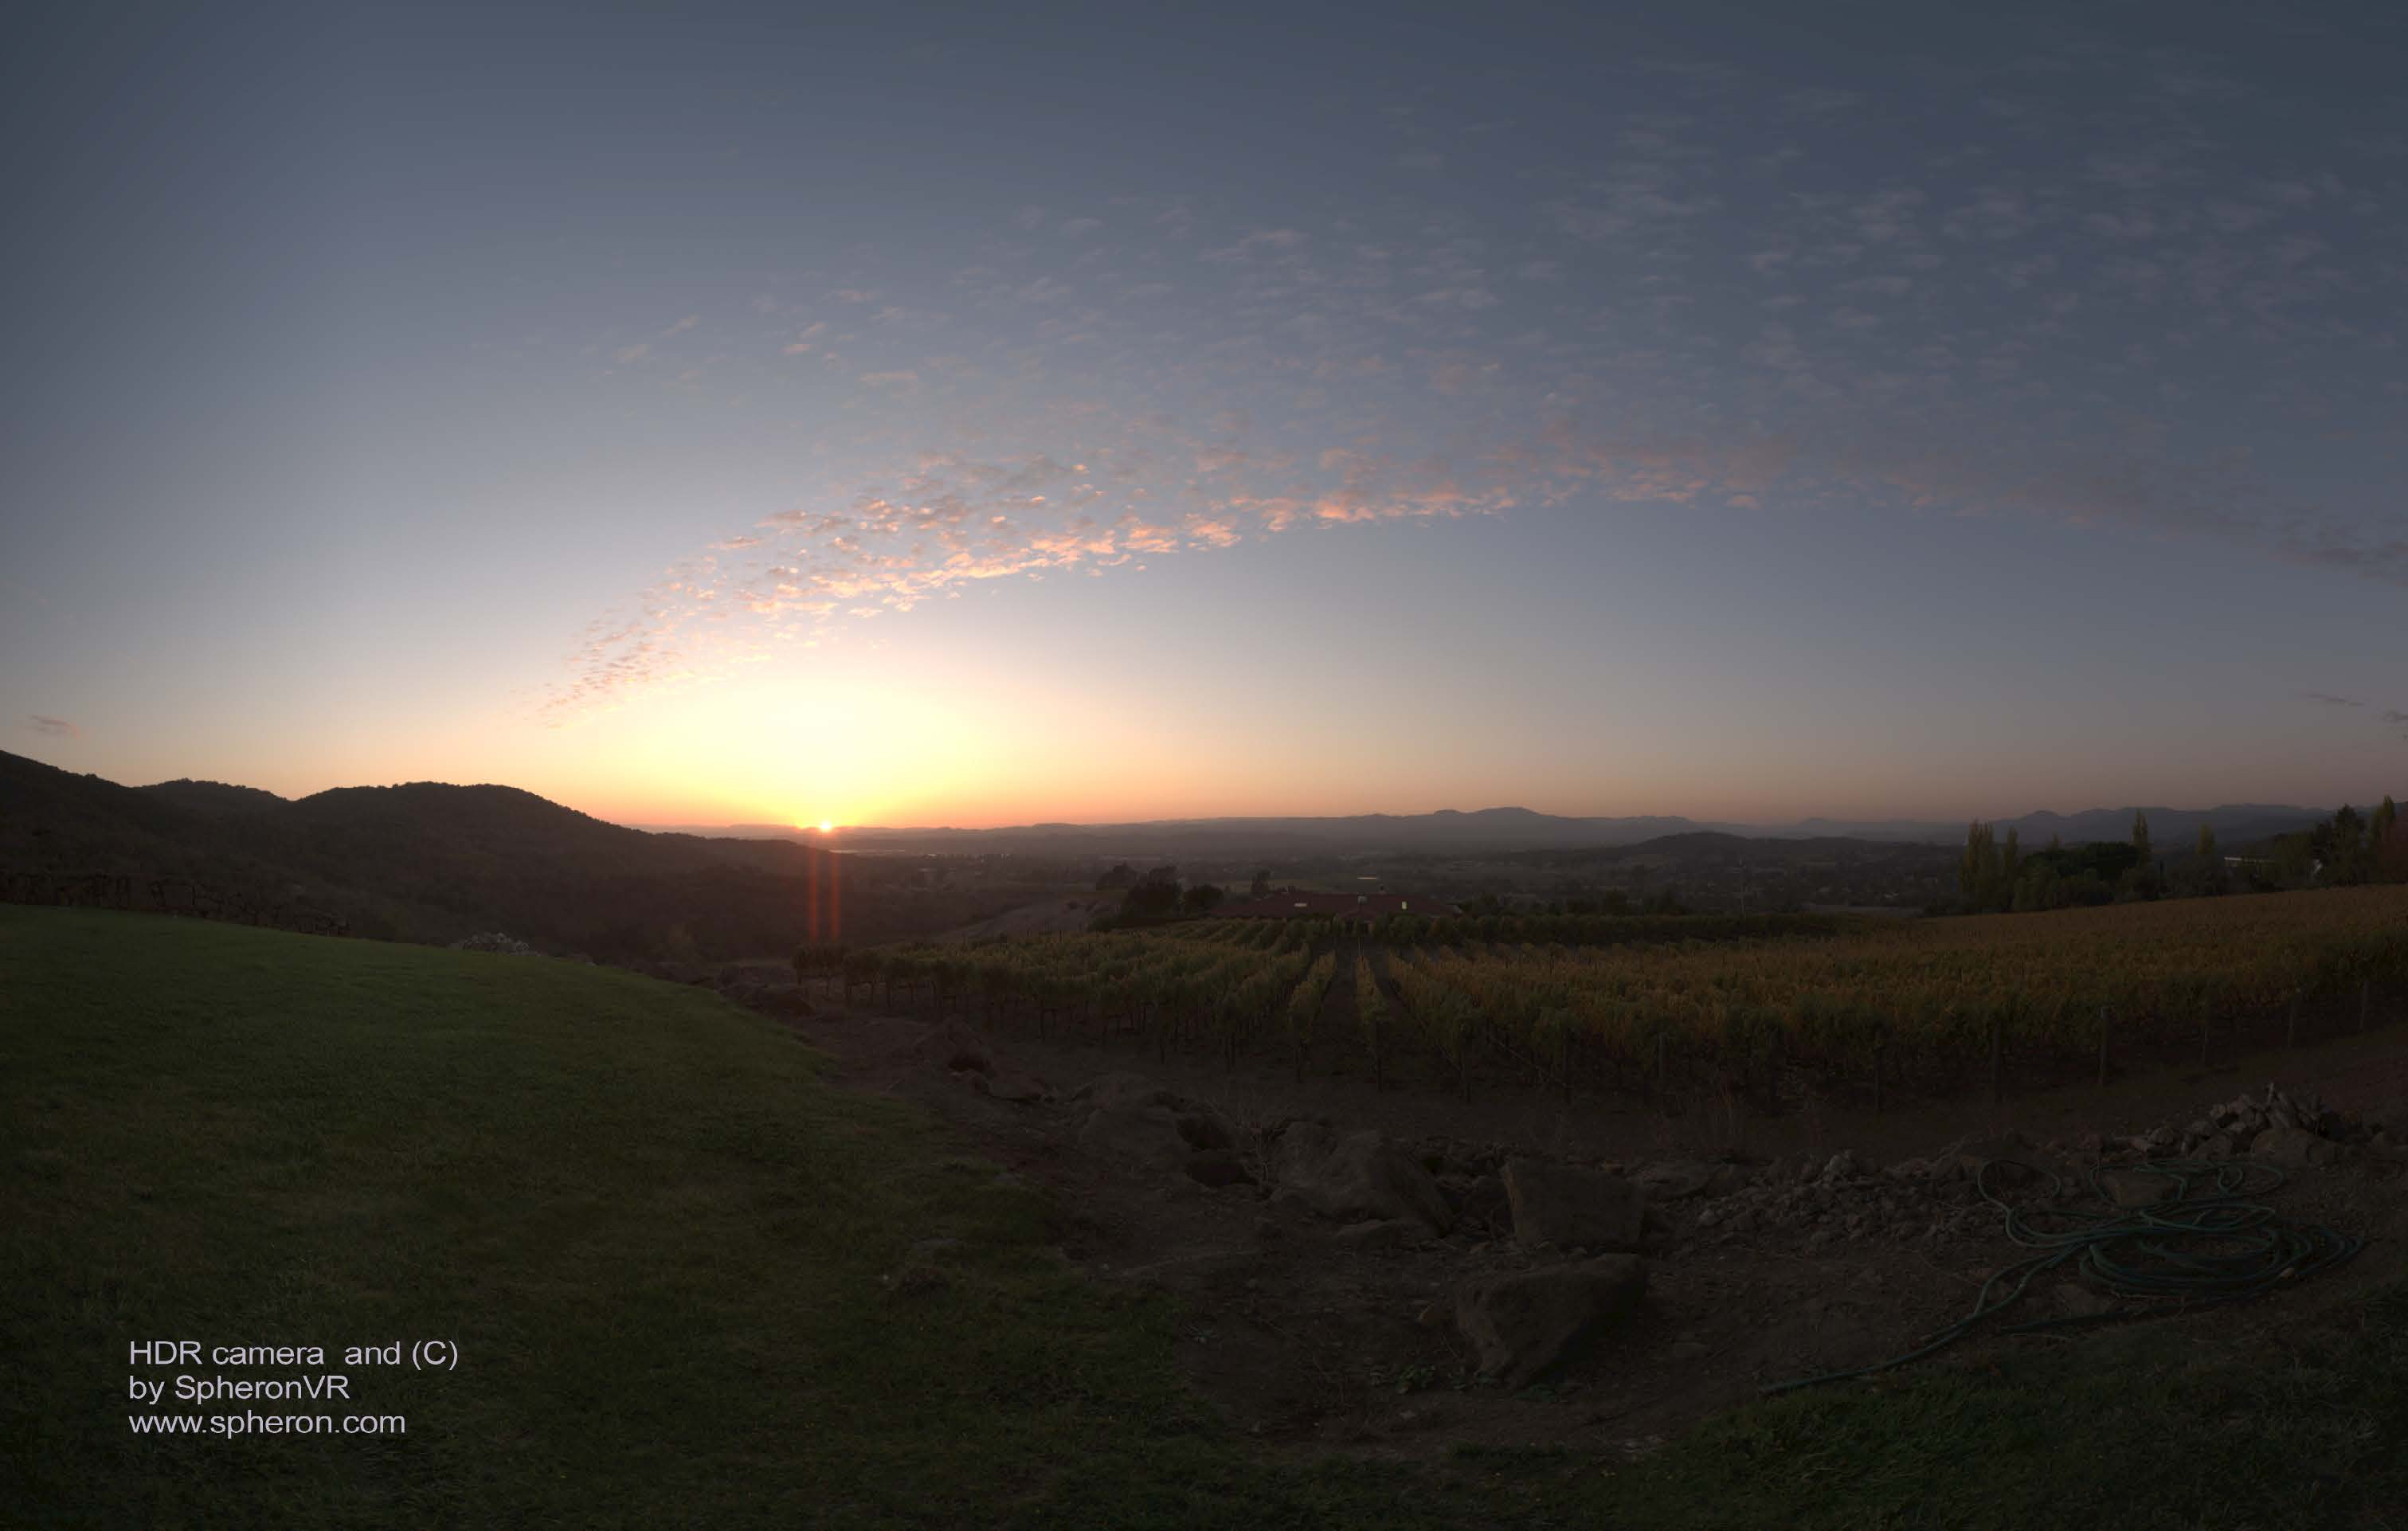
\includegraphics[height=14em]{images/valley_original.jpg}
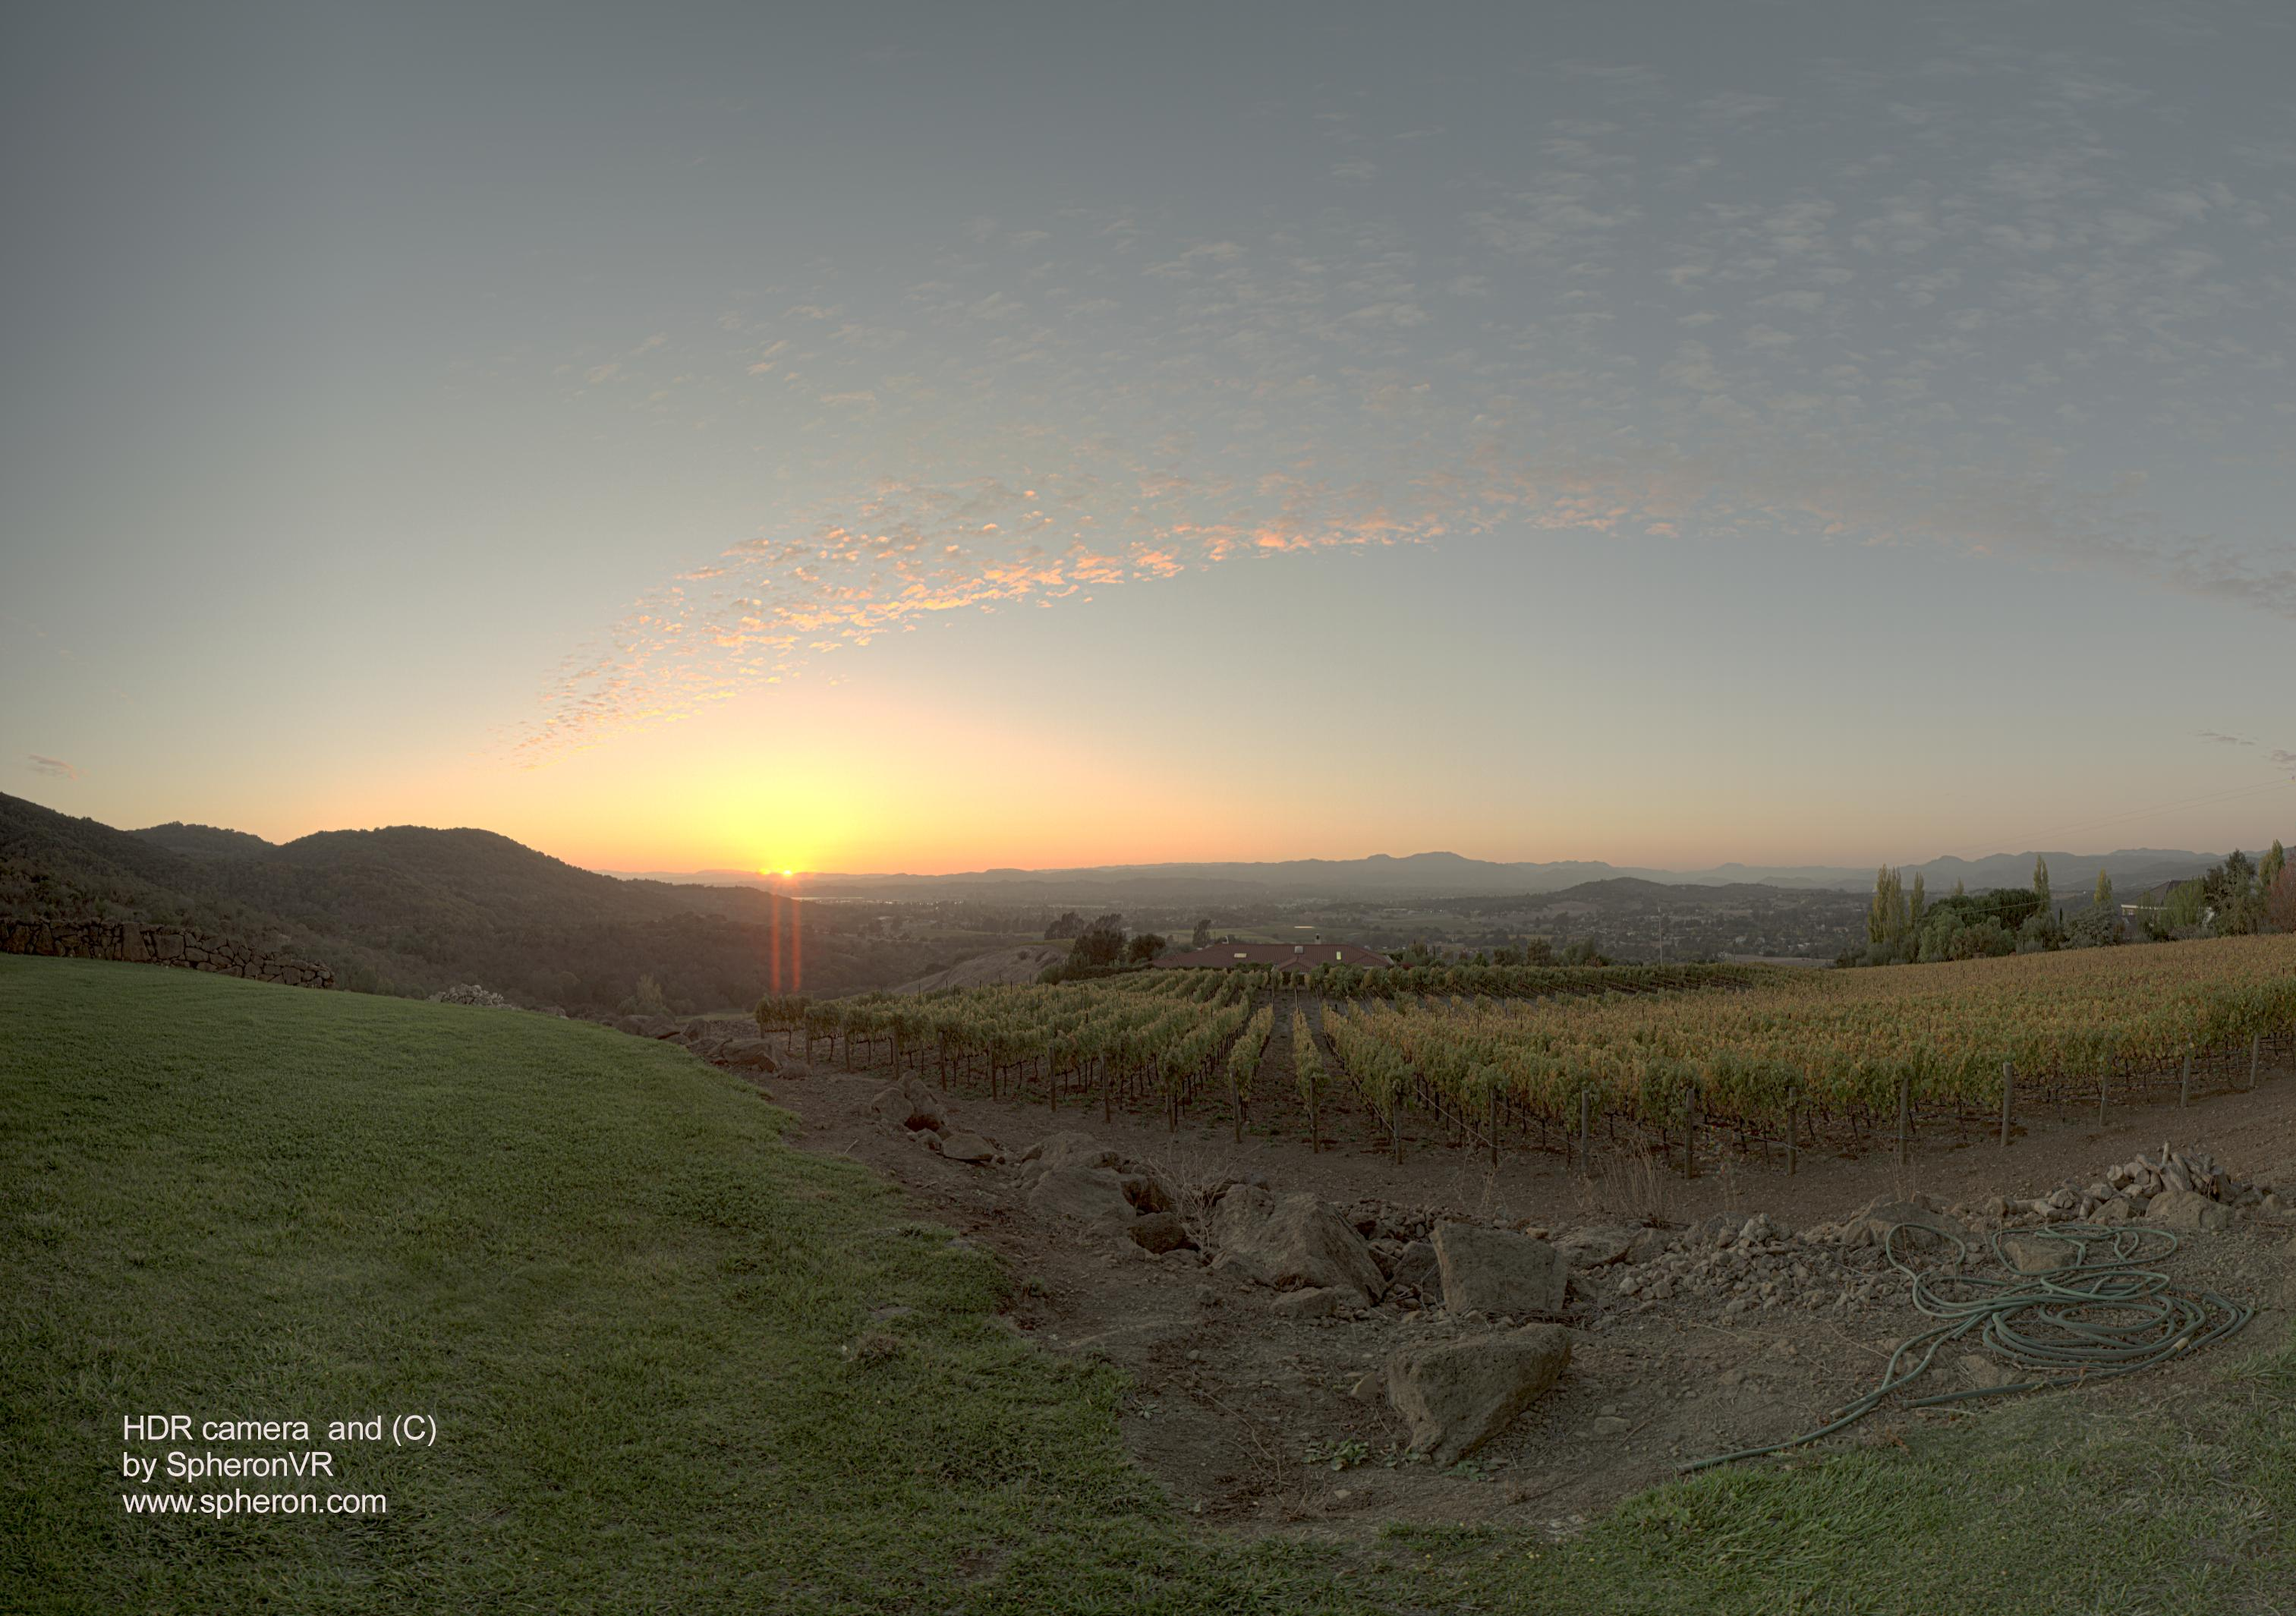
\includegraphics[height=14em]{images/valley_processed.jpg}
\end{center}
\caption{HDR image rendering 2}
\label{example2}
\end{figure}

\begin{figure}[H]
\begin{center}
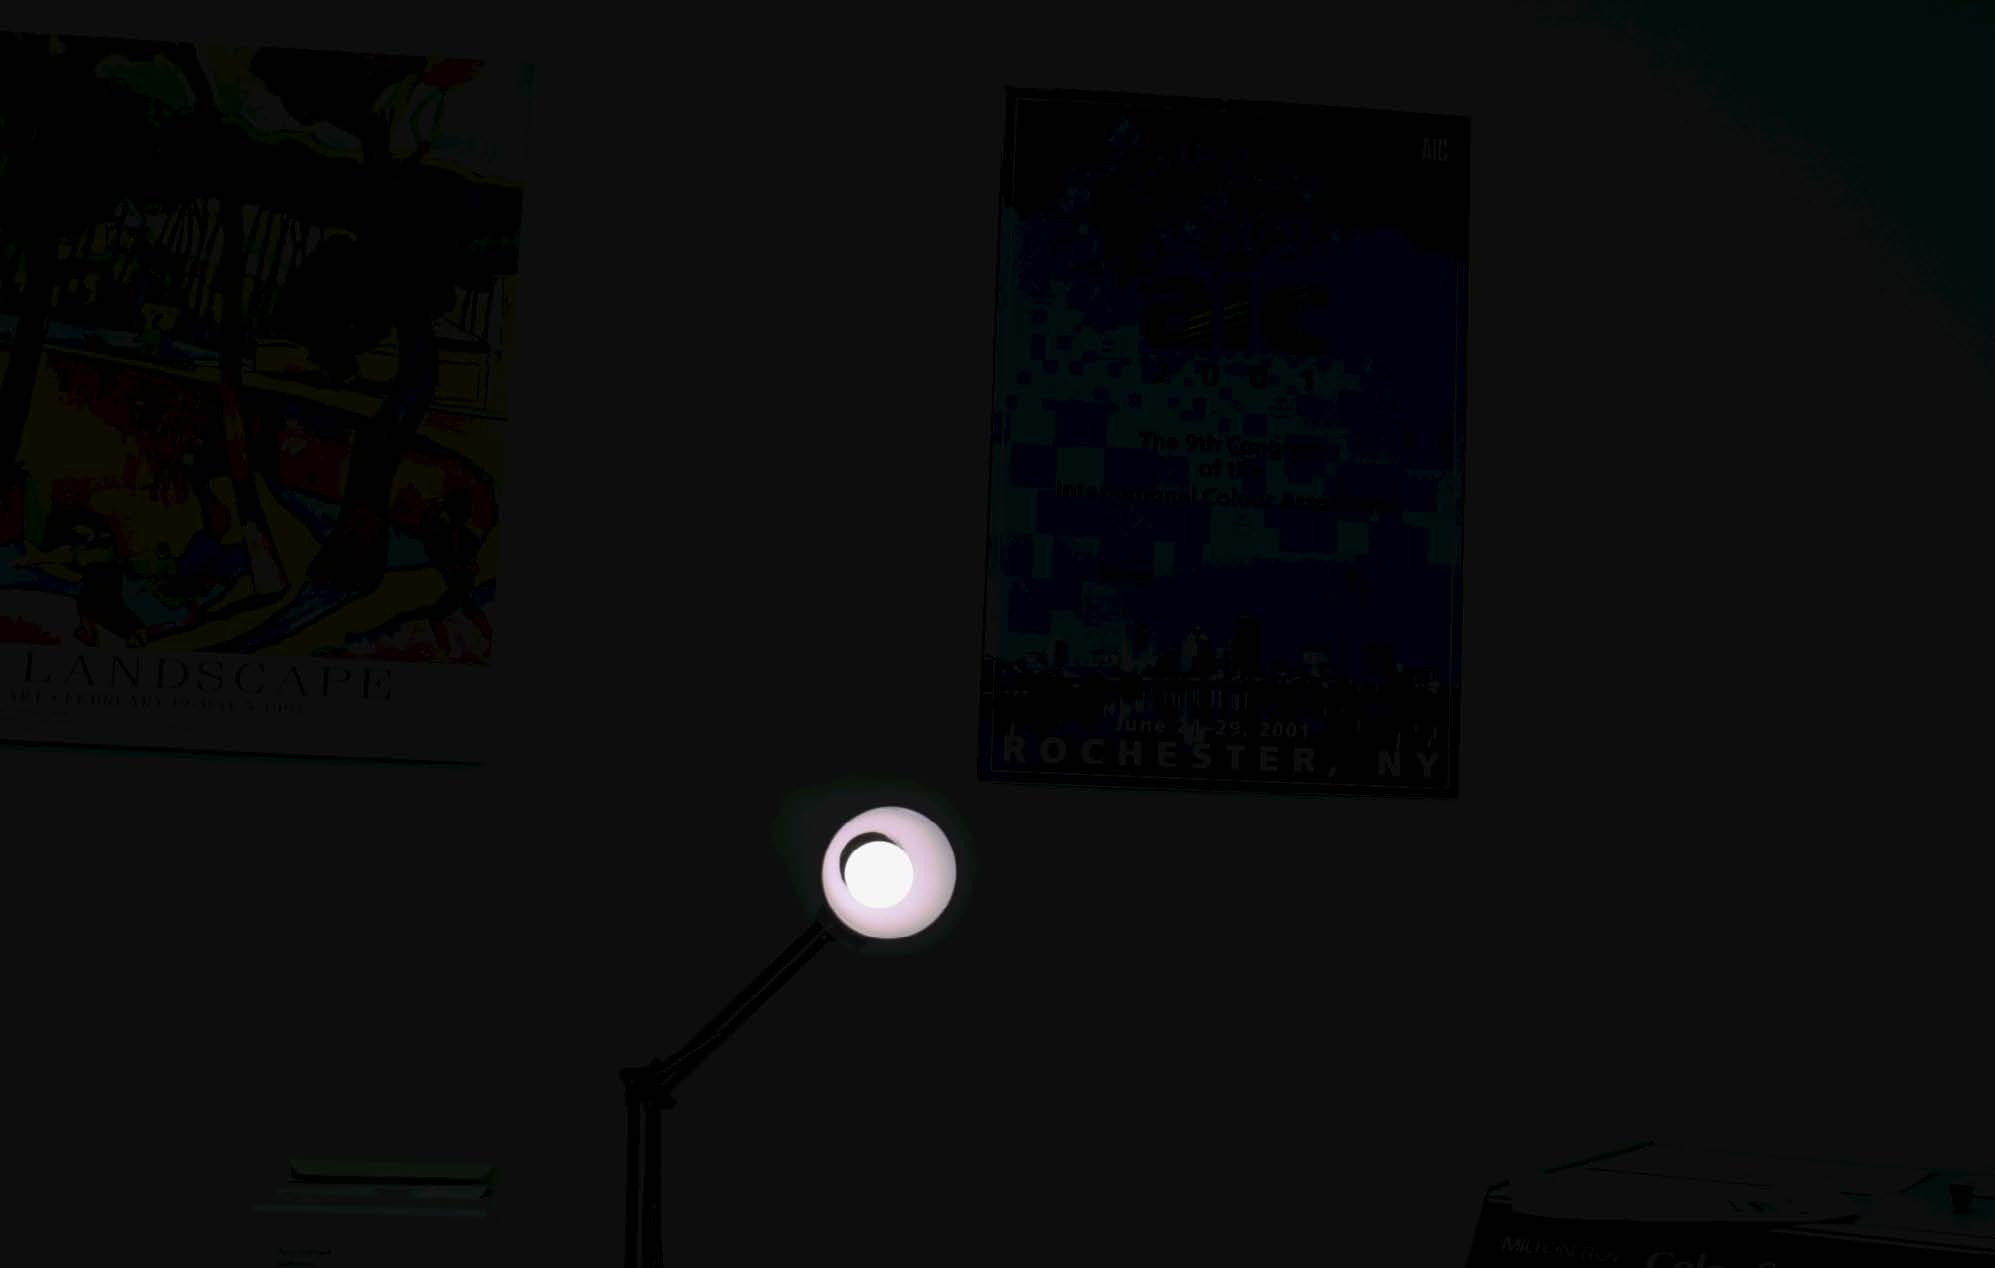
\includegraphics[height=14em]{images/wall_original.jpg}
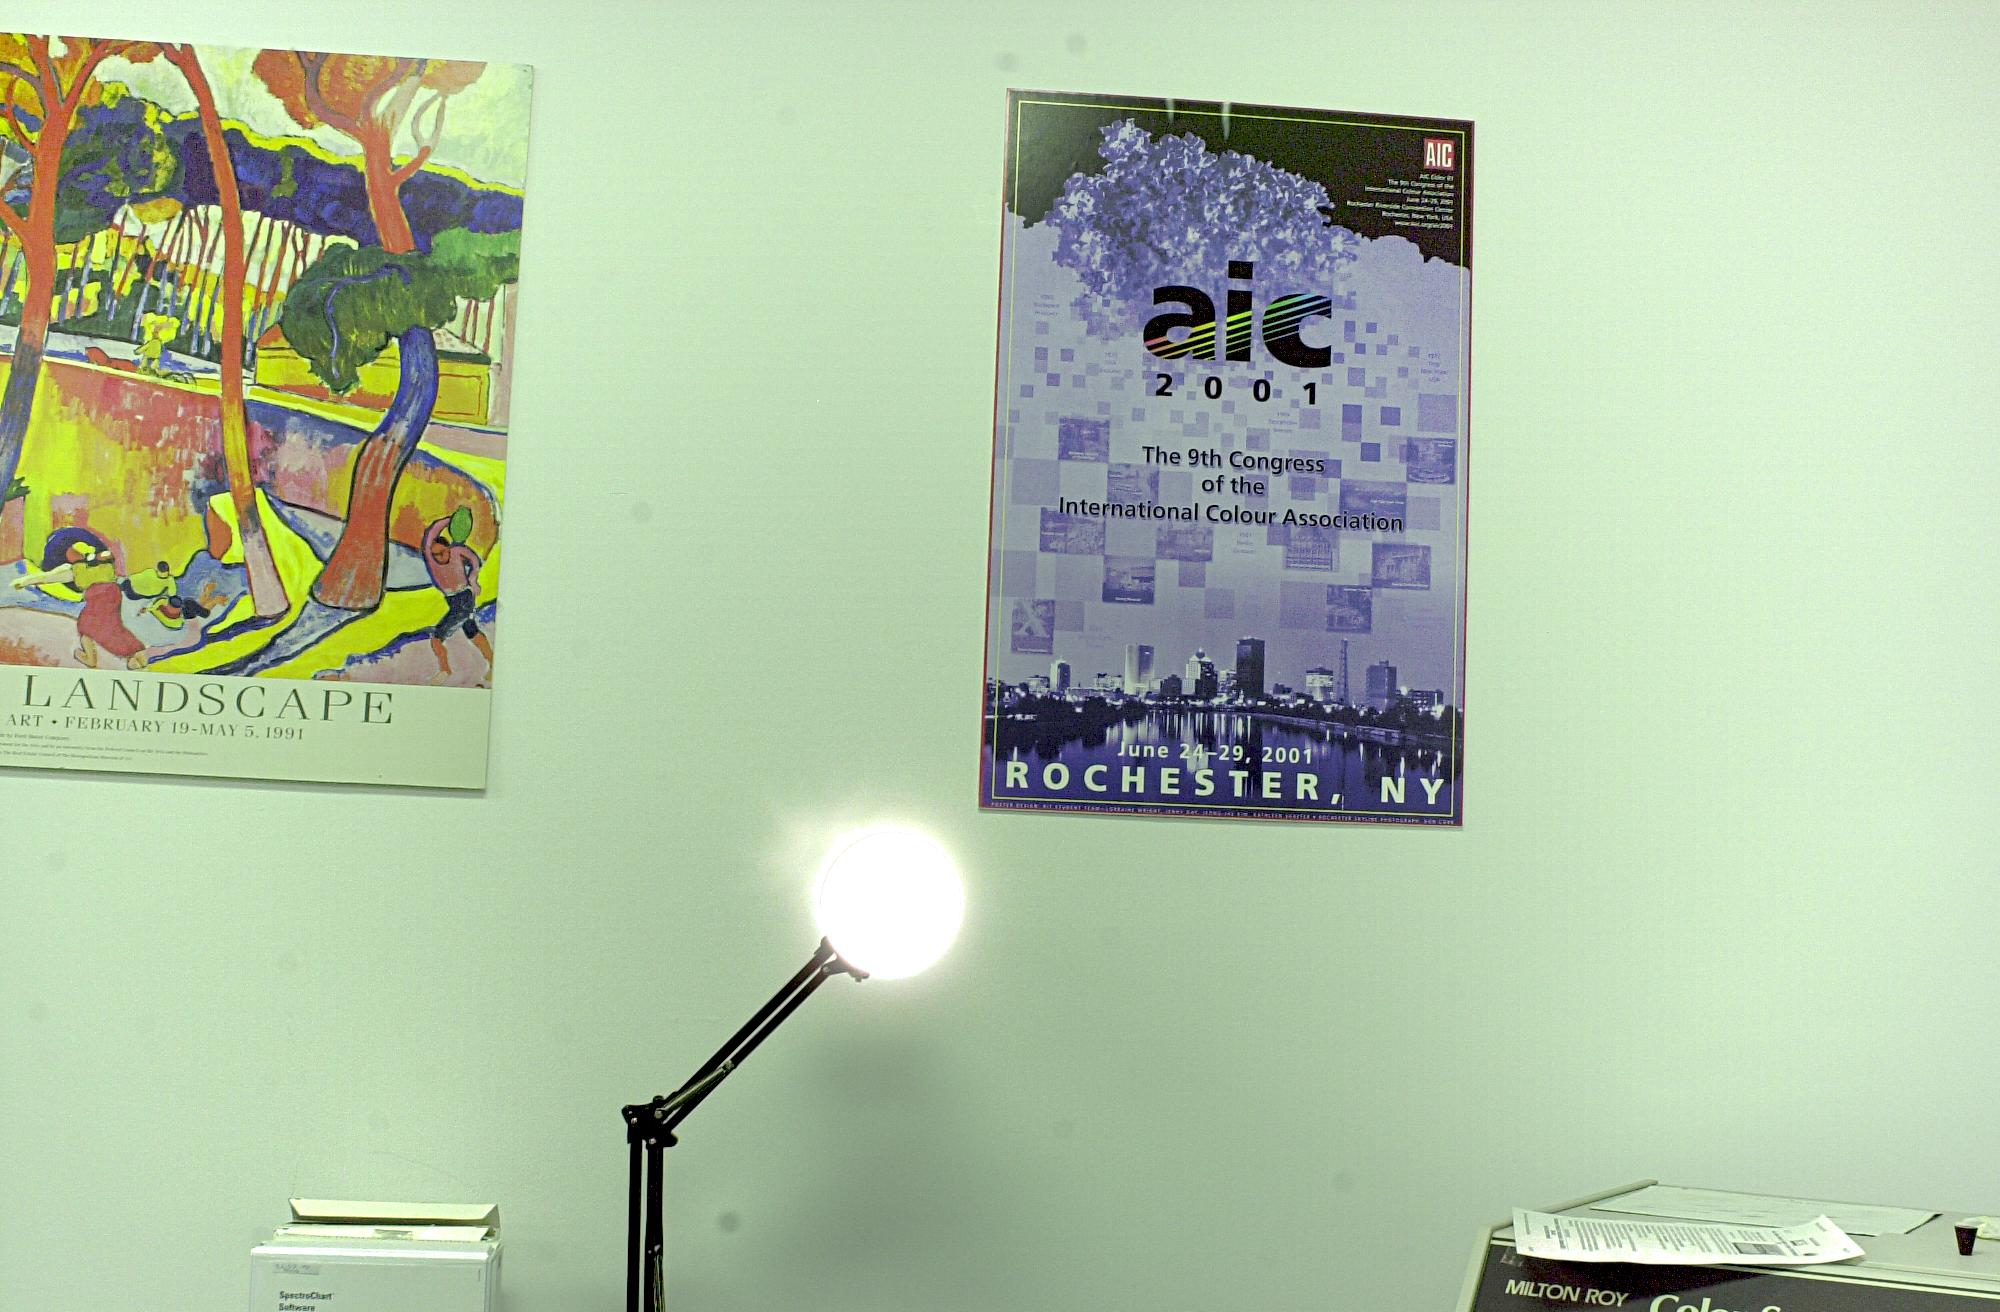
\includegraphics[height=14em]{images/wall_processed.jpg}
\end{center}
\caption{HDR image rendering 3}
\label{example2}
\end{figure}

Different parameters are used based on different natural scenes. Above results indicate that iCAM06 extends the previous model iCAM, to a large luminance levels ranging from low scotopic to high luminance photopic levels. Details in both bright and dark areas of these image are preserved.

\section{Conclusion}
Experimental results show that the refined iCAM06 model is able to handle HDR image rendering in both indoor and outdoor scenes, and it is capable of keeping as many as details in both bright and dark areas in the natural scenes. The iCAM06 make predictions based on human eye perception, which can guarantee that HDR rendering reproduce an LDR image which is same with original scene with wide range of luminance. With the help of iCAM06, people can use advanced image capturing device to capture splendid natural landscape and others are able to see this magnificent scenery just sit in the front of computer like they are in the real place without losing any details. 
\section*{Acknowledgments}
Adapting the code provided by the authors of Jiangtao Kuang, Garrett M. Johnson, Mark D. Fairchild

{
\small
\bibliographystyle{unsrt}
\bibliographystyle{ieee}
\bibliography{references} % Create file refs.bib, and run bibtex.
}

\end{document}
